\chapter{Architeture of Data Converters}
\addborderb
\label{chapter:architecture}
\section{DAC Architecture}
\label{sec:dac_architecture}
DAC Architecture use varius techniques to convert digital signals to analog signals.
Some use voltage division, whereas others employ current
steering and even charge scaling to map the digital value into an analog quantity

\subsection{Resistor stringstyle DAC}
The resistor-string DAC, shown in Fig. \ref{fig:resistor_style}(a) uses 2N identical resistors and switches to divide voltage at selected taps, ensuring monotonic output. However, parasitic capacitance at the output node limits speed for higher resolutions. Fig. \ref{fig:resistor_style}(b) improves speed using a binary switch array, reducing the number of active switches. While compact designs are possible with active resistors, higher resolutions demand precise resistor values, balancing area and power dissipation.
The value of the output voltage is given by the equation \ref{eq:resistor_string_dac}
\begin{equation}
\label{eq:resistor_string_dac}
	V_{i,\text{ideal}} = \left( \frac{i V_{\text{REF}}}{2^N} \right), \quad \text{for } i = 0, 1, 2, \ldots, 2^N - 1
\end{equation}

\begin{center}
\begin{table}[H]
	\centering
	\label{tab:3bit_dac_output}
	\begin{tabular}{ccc|c}
		$D_2$ & $D_1$ & $D_0$ & $v_{\text{OUT}}$ \\
		\hline
		0 & 0 & 0 & 0 \\
		0 & 0 & 1 & 0.625 \\
		0 & 1 & 0 & 1.25 \\
		0 & 1 & 1 & 1.875 \\
		1 & 0 & 0 & 2.5 \\
		1 & 0 & 1 & 3.125 \\
		1 & 1 & 0 & 3.75 \\
		1 & 1 & 1 & 4.375 \\
	\end{tabular}
	\caption{Output voltages generated from the 3-bit DAC}
\end{table}
\end{center}
\begin{figure}[H]
	\centering
	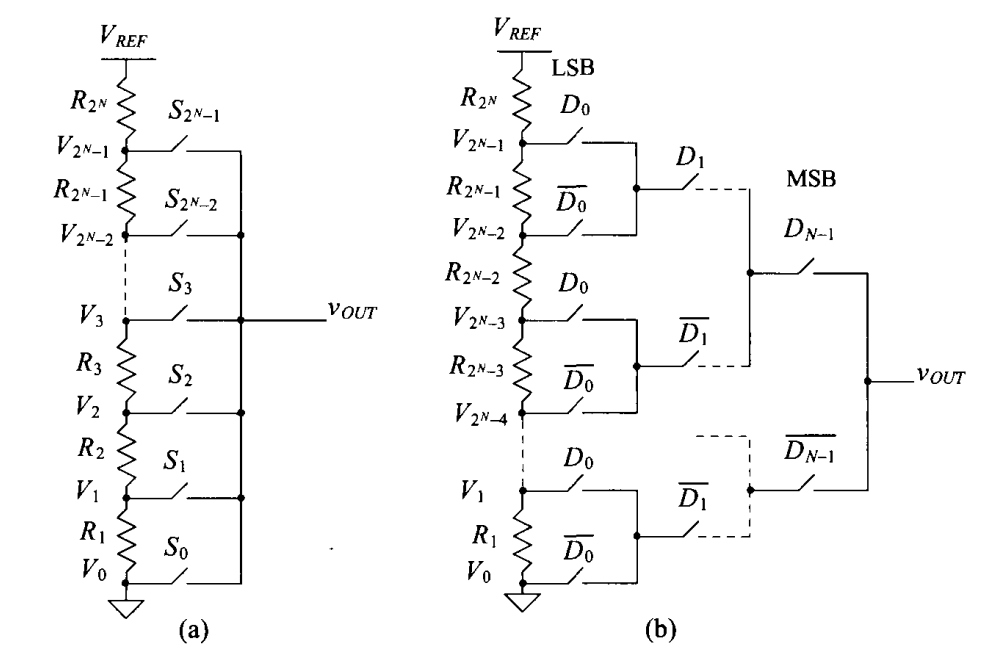
\includegraphics[width=0.7\textwidth]{figs/resistor_style.png}
	\caption{(a) A simple resistor-string DAC and (b) The use of a binary switch
array to lower the output capacitance}
	\label{fig:resistor_style}
	\vspace{0.5cm}
\end{figure}
\subsection{R-2R Ladder DAC}
The R-2R ladder DAC, shown in Fig. \ref{fig:r2r_dac}, employs a network of resistors alternating between values of R and 2R. This configuration ensures binary-weighted voltage division at each node, as illustrated in Fig. \ref{fig:r2r_dac}. The digital input switches each resistor to either ground or the inverting input of the op-amp, maintaining constant node voltages. The total current from the reference voltage remains constant, ensuring stable operation for varying digital inputs.
The output voltage, $v_{\text{OUT}}$, depends on currents flowing through the feedback resistor, $R_F$, such that
\begin{equation}
v_{\text{OUT}} = -i_{\text{TOT}} \cdot R_F \tag{29.14}
\end{equation}
where $i_{\text{TOT}}$ is the sum of the currents selected by the digital input, given by
\begin{equation}
i_{\text{TOT}} = \sum_{k=0}^{N-1} D_k \cdot \frac{V_{\text{REF}}}{2^{N-k}} \cdot \frac{1}{2R} \tag{29.15}
\end{equation}
where $D_k$ is the $k$-th bit of the input word with a value that is either a 1 or a 0.
\begin{figure}[H]
	\centering
	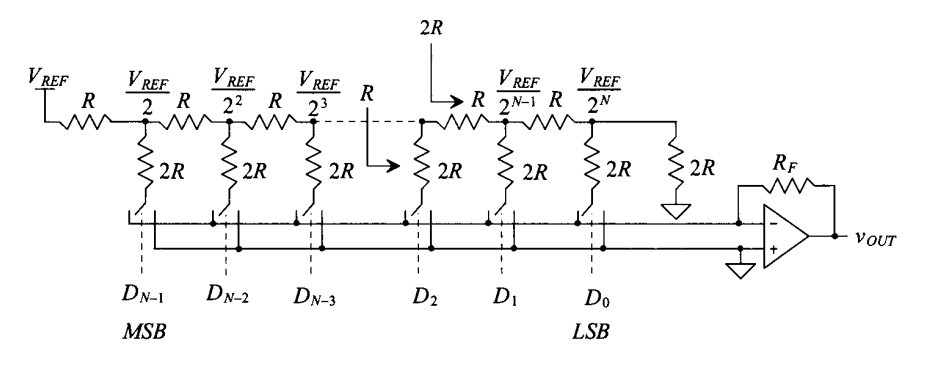
\includegraphics[width=0.5\textwidth]{figs/r2r_dac.png}
	\caption{A R-2R ladder digital-to-analog converter architecture}
	\label{fig:r2r_dac}
	\vspace{0.5cm}
\end{figure}
\subsection{Current Steering DAC}
Current steering DACs, shown in Fig. \ref{fig:current_steering_dac}, utilize a network of current sources to generate an output voltage proportional to the digital input rather then as in previous DAC where voltage was converted into current which generated voltage at the output. The current sources are controlled by switches that connect them to either the reference voltage or ground, allowing for precise control over the output current. This architecture is particularly effective for high-speed applications due to its fast switching capabilities and low output capacitance.
\begin{figure}
	\centering
	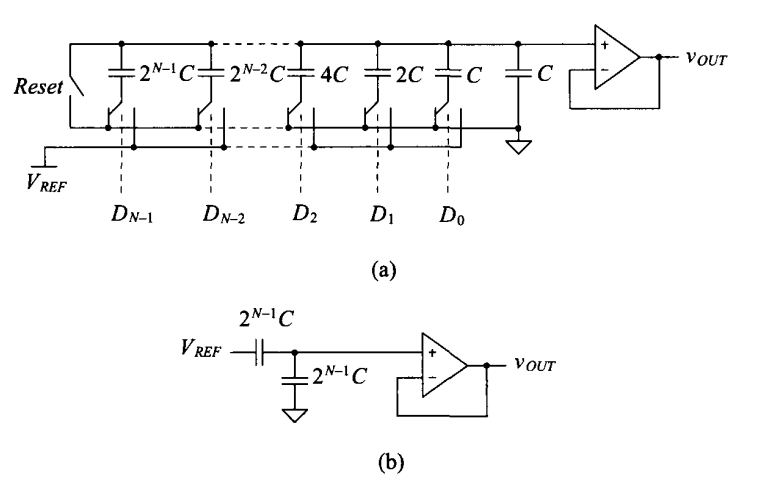
\includegraphics[width=0.7\textwidth]{figs/current_steering_dac.png}
	\caption{A current steering digital-to-analog converter architecture}
	\label{fig:current_steering_dac}
	\vspace{0.5cm}
\end{figure}
\subsection{Charge Scaling DAC}
The charge-scaling DAC, shown in Fig. \ref{fig:charge_scaling_dac}, employs a parallel array of binary-weighted capacitors connected to an op-amp. The capacitors are initially discharged, and the digital input switches each capacitor to either $V_{\text{REF}}$ or ground, creating an output voltage proportional to the digital input. This architecture is compact and efficient, making it suitable for applications requiring low power and high precision.

The output voltage, $v_{\text{OUT}}$, is given by:
\begin{equation}
v_{\text{OUT}} = \sum_{k=0}^{N-1} D_k \cdot 2^{k-N} \cdot V_{\text{REF}}
\end{equation}
where $D_k$ is the $k$-th bit of the digital input word, $V_{\text{REF}}$ is the reference voltage, and $N$ is the number of bits.

\begin{figure}[H]
	\centering
	\includegraphics[width=0.7\textwidth]{figs/charge_scaling_dac.png}
	\caption{(a) A charge-scaling DAC, (b) the equivalent circuit with the MSB = 1,and all other bits set to zero.}
	\label{fig:charge_scaling_dac}
	\vspace{0.5cm}
\end{figure}
\subsection{Cyclic DAC}
The cyclic DAC, shown in Fig. \ref{fig:cyclic_dac}, uses a minimal set of components to perform digital-to-analog conversion. It operates by processing one bit at a time in a serial fashion, requiring $N$ cycles for an $N$-bit conversion. The architecture employs a summer, a sample-and-hold (S/H) circuit, and an amplifier with a gain of 0.5. The summer adds $V_{\text{REF}}$ or ground to the feedback signal based on the input bits, while the amplifier feeds the output voltage back to the summer for the next cycle.

The output voltage at the end of the $n$-th cycle is given by:
\begin{equation}
v_{\text{OUT}}(n) = \left( D_{N-1} \cdot V_{\text{REF}} + \frac{1}{2} \cdot v_A(n-1) \right) \cdot \frac{1}{2}
\end{equation}
where $D_{N-1}$ is the most significant bit of the input word, $v_A(n-1)$ is the output voltage from the previous cycle, and $v_{\text{OUT}}(0)$ is initialized to zero.

This architecture is advantageous for its simplicity and ease of implementation using switched capacitors. However, its accuracy depends on the precision of the amplifier and the sample-and-hold circuit.

\begin{figure}[H]
	\centering
	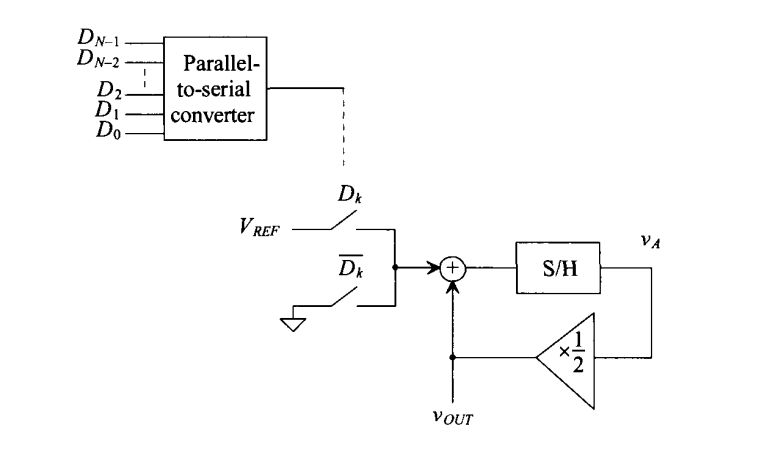
\includegraphics[width=0.7\textwidth]{figs/cyclic_dac.png}
	\caption{A cyclic digital-to-analog converter architecture}
	\label{fig:cyclic_dac}
	\vspace{0.5cm}
\end{figure}
\subsection{Pipline DAC}
The pipeline DAC, shown in Fig. \ref{fig:pipeline_dac}, extends the cyclic DAC architecture by employing multiple stages, each responsible for processing one bit of the digital input. This configuration allows for continuous operation, as each stage processes a new bit while passing the intermediate result to the next stage. The architecture consists of sample-and-hold (S/H) circuits, summers, and amplifiers with a gain of 0.5.

The output voltage at the $n$-th stage is given by:
\begin{equation}
v_{\text{OUT}}(n) = \left( D_{n-1} \cdot V_{\text{REF}} + v_{\text{OUT}}(n-1) \right) \cdot \frac{1}{2}
\end{equation}
where $D_{n-1}$ is the bit processed by the $n$-th stage, $v_{\text{OUT}}(n-1)$ is the output voltage from the previous stage, and $v_{\text{OUT}}(0)$ is initialized to zero.

This architecture is advantageous for its high throughput, as it produces one output per clock cycle after an initial delay of $N$ cycles. However, it requires precise amplifier gains and increased circuitry compared to cyclic DACs.

\begin{figure}[H]
	\centering
	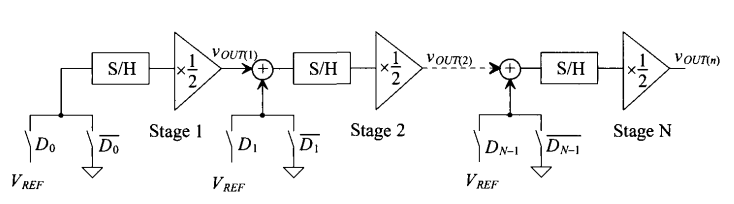
\includegraphics[width=0.7\textwidth]{figs/pipeline_dac.png}
	\caption{A pipeline digital-to-analog converter architecture}
	\label{fig:pipeline_dac}
	\vspace{0.5cm}
\end{figure}
\section{ADC Architecture}
\label{sec:adc_architecture}
ADC Architecture use various techniques to convert analog signals to digital signals.
Some use voltage division, whereas others employ current
steering and even charge scaling to map the analog value into a digital quantity.
\subsection{Flash ADC}
The flash ADC, shown in Fig. \ref{fig:flash_adc}, is the fastest type of ADC architecture. It uses a resistor-string DAC to divide the reference voltage into $2^N$ levels, where $N$ is the resolution of the ADC. Each level is fed into a comparator, which compares the input voltage with the reference levels and generates a thermometer code. The thermometer code is then converted into a binary digital output using a decoder.

The flash ADC requires $2^N - 1$ comparators and $2^N$ resistors, making it area-intensive for higher resolutions. However, its speed is unmatched, as it performs the conversion in a single clock cycle. The disadvantages of the flash ADC include high power consumption and increased complexity for higher resolutions.

\begin{figure}[H]
	\centering
	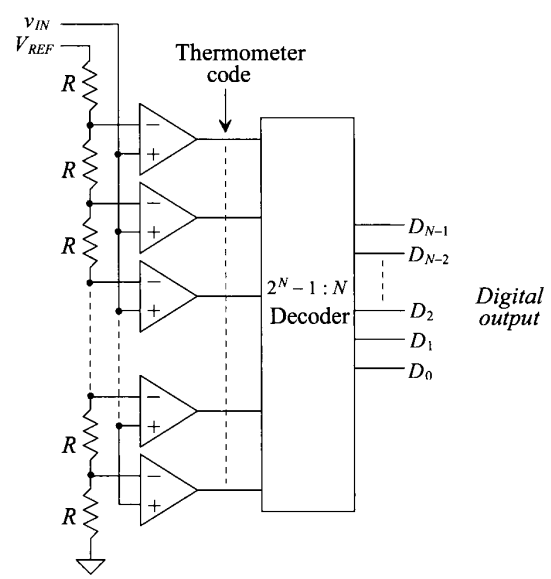
\includegraphics[width=0.7\textwidth]{figs/flash_adc.png}
	\caption{Block diagram of a Flash ADC architecture}
	\label{fig:flash_adc}
	\vspace{0.5cm}
\end{figure}
\subsection{Successive Approximation Register (SAR) ADC}
The successive approximation register (SAR) ADC, shown in Fig. \ref{fig:sar_adc}, performs analog-to-digital conversion using a binary search algorithm. It employs a sample-and-hold (S/H) circuit, a comparator, a digital-to-analog converter (DAC), and a successive approximation register (SAR). The SAR controls the DAC output based on the comparator's feedback, iteratively refining the digital output.

The conversion process begins by sampling the input voltage, $v_{\text{IN}}$, and initializing the SAR to its midpoint value. The comparator compares $v_{\text{IN}}$ with the DAC output, adjusting the SAR value accordingly. This process repeats for $N$ cycles, where $N$ is the resolution of the ADC, producing the final digital output.

The SAR ADC is advantageous for its balance between speed and power consumption, making it suitable for medium-speed applications. However, its accuracy depends on the precision of the DAC and comparator.

\begin{figure}[H]
	\centering
	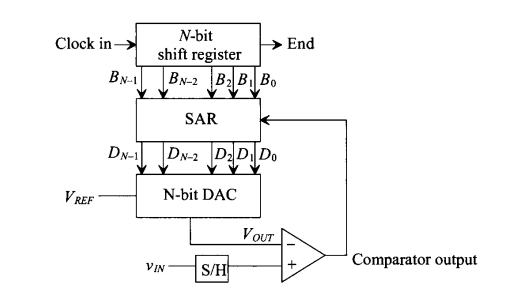
\includegraphics[width=0.8\textwidth]{figs/sar_adc.png}
	\caption{Block diagram of a Successive Approximation Register (SAR) ADC architecture}
	\label{fig:sar_adc}
	\vspace{0.5cm}
\end{figure}
\subsection{Pipeline ADC}
The pipeline ADC, as illustrated in Fig.~\ref{fig:pipeline_adc}, achieves high throughput by dividing the conversion process into multiple stages, each resolving a single bit (or a few bits) per stage. Each stage typically consists of a sample-and-hold (S/H) circuit, a 1-bit ADC (comparator), a digital-to-analog sub-converter (DAC), a subtractor, and a gain stage (usually by 2). The residue from each stage is passed to the next, allowing pipelined operation.

The operation of each stage is as follows:
\begin{enumerate}
	\item The input signal is sampled and compared to $\frac{V_{\text{REF}}}{2}$ by the 1-bit ADC.
	\item If $v_{\text{IN}} > \frac{V_{\text{REF}}}{2}$, the comparator outputs 1; otherwise, it outputs 0. The corresponding reference ($0$ or $\frac{V_{\text{REF}}}{2}$) is subtracted from the input to generate the residue.
	\item The residue is amplified by 2 and passed to the next stage.
\end{enumerate}

After an initial latency of $N$ clock cycles (for an $N$-stage pipeline), the converter outputs one result per clock cycle, making it suitable for high-speed applications. The main trade-offs are increased circuit complexity and the need for precise inter-stage gain and timing.

\begin{figure}[H]
	\centering
	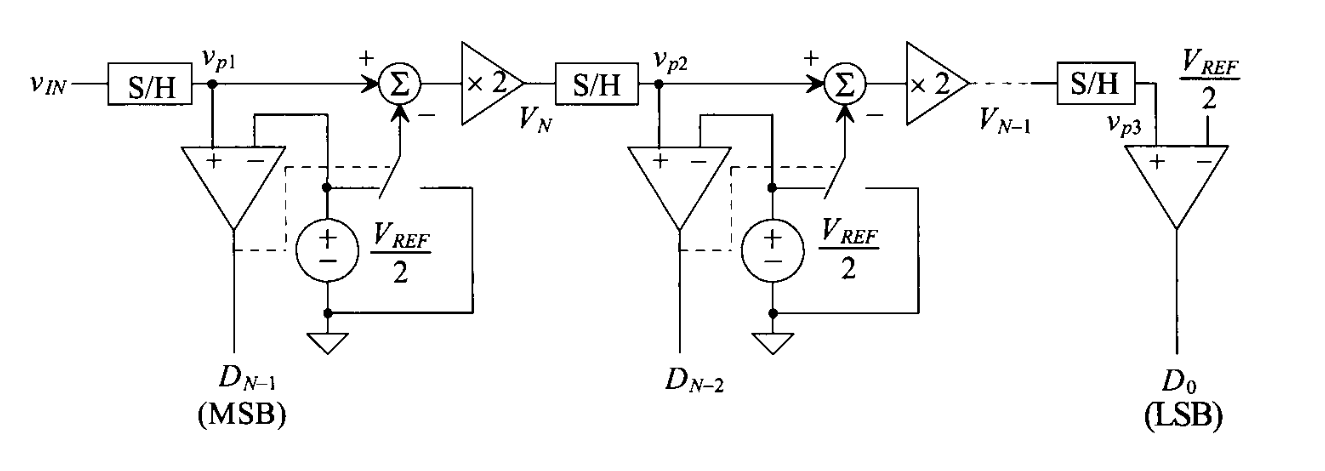
\includegraphics[width=0.8\textwidth]{figs/pipeline_adc.png}
	\caption{Block diagram of a pipeline ADC architecture}
	\label{fig:pipeline_adc}
	\vspace{0.5cm}
\end{figure}
